\section{Implementation on Software-defined radio}
\label{sec:implementation_on_SDR}

\begin{figure}[t]
    \centerline{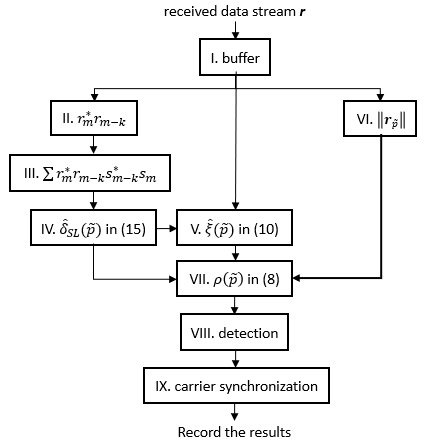
\includegraphics[width=2.7in,height=2.6in]{SDR_receiver_new.png}}
    \caption{Block diagram for implementing the proposed algorithm in TBB}
    \label{fig:SDR_receiver}
    \end{figure}

% To make our proposed algorithm work at a very high sample rate,
% the first improvement of algorithm is by using pipeline.
% Threading Building Blocks (TBB) is a well-known C++
% library that enables parallel programming on multicore processor~\cite{Michael_19}.
To demonstrate the practicality of our algorithms, we have implemented them in C++ on a general
purpose processor (GPP). The different aspects of the algorithm are mapped to logical nodes in a pipelined, parallel processing atchitecture
using Threading Building Blocks (TBB)~\cite{Michael_19}.

Figure~\ref{fig:SDR_receiver} shows a simple block diagram illustrating pipeline for the algorithm.
Due to space constraints, we don't give the details of each node.
It is necessary to discuss the node for computing the phasor estimate $\hat{\xi}$ (node V). 
The numerator of~\eqref{eq:opt_xi} performs a time-varying convolution, which cannot be computed efficiently via FFT.
Our solution to increasing the computational efficiency is to use parallel programming 
of TBB. Specifically,~\eqref{eq:opt_xi} can be computed in three stages:
1. Compute several segments of $\sum r_ns_n^*$ in several nodes in parallel;
2. each node is then multiplied by $\hat{\delta}_{SL}$ at the middle index of the 
partial correlation.
3. Sum all the nodes together.
Thus, \eqref{eq:opt_xi} is computed more efficiently as

\begin{equation}
    \label{eq:refined_opt_S}
    ||\bm{s}||^2\cdot\hat{\xi} \approx \sum_{i=0}^{L-1} e^{-j\pi \hat{\delta}\frac{N(2m+1)}{L}}
    \sum_{n=mN/L}^{(m+1)N/L-1}r_ns_n^*,
  \end{equation}
where $L$ is the number of nodes. Thus, by using parallel pro-gramming,
the efficiency of computing $\hat{\xi}$ is increased by $L^2$.

Now we show the results of the proposed algorithm in parallel programming on SDR.
The signal are transmitted and received between two universal software radio peripheral (USRP)
connected by a 5-Gigabit Ethernet cable to laptops. At the receiver side, 
the CPU includes 6 cores and 12 threads with 4.5 GHz clock frequency. The results of 
Google benchmark for each node in Figure~\ref{fig:SDR_receiver}
are shown in Table~\ref{table:BM_function_nodes}. Note, the time cost in the table
refers to one buffer size of 8192 samples. The throughput of the 
pipeline is dominated by the node with the longest time. Thus, the ideal throughput is approximately equal to
$8192/837253 \cdot 10^3 \approx 9.78$ MHz.

In operation, the throughput of the algorithm is in the range of 4.5 MS/s $\sim$ 5.0 MS/s with latency near 1 ms;
The detection algorithm is very robust and the false alarm probability is near 0 at moderate SNR.

\begin{table}[t]
    \caption{Benchmark results of nodes in Figure~\ref{fig:SDR_receiver} with buffer size 8192}  % title of Table
    \centering % used for centering table
    \begin{tabular}{c c c c} % centered columns (4 columns)
    \hline\hline %inserts double horizontal lines
    Node name & Time (ns) & CPU (ns) & Iterations \\ [0.5ex] % inserts table
    %heading
    \hline % inserts single horizontal line
    I. Buffer  & 408721 & 407754 & 1703 \\ % inserting body of the table
    II. $r_m^*r_{m-k}$  & 160069 & 160054 & 3416 \\
    III. $r_m^*r_{m-k}s_{m-k}^*s_m$ & 498967 & 498876 & 1471 \\
    IV. $\hat{\delta}_{SL}^{(1)}$ & 187135 & 187121 & 3602 \\
    V. $\hat{\xi}$ & 780620 & 780523 & 886 \\
    VI. $||\bm{r}||$ & 203907 & 203892 & 3416 \\ % [1ex] adds vertical space
    VII. $\rho(p)$ & 837253 & 837048 & 829 \\
    VIII. detection & 378793 & 378765 & 1844 \\
    IX. carrier synchronization & 811747 & 811739 & 844  \\ [1ex]
    \hline
    \end{tabular}
    \label{table:BM_function_nodes} % is used to refer this table in the text
  \end{table}

